\documentclass[journal]{IEEEtran}
\usepackage{graphicx}
\usepackage{array}
\usepackage{subfigure}
\usepackage{adjustbox}

\ifCLASSINFOpdf
  % \usepackage[pdftex]{graphicx}
  % \DeclareGraphicsExtensions{.pdf,.jpeg,.png}
\else
  % \DeclareGraphicsExtensions{.eps}
\fi

%\hyphenation{op-tical net-works semi-conduc-tor}

\begin{document}
\title{Delivering Reliable Software in the European Scientific Arena: Evolution of Methodologies and New Trend Analysis}
%\title{15 years of European scientific software development: evolution and methodologies}

\author{E. Ronchieri,
        P. Orviz Fernandez,
        M. David,
	D. C. Duma,
        J. Gomes,
        D. Salomoni
\thanks{D. C. Duma, E. Ronchieri, and D. Salomoni are with INFN - CNAF, Bologna, Italy.}
\thanks{P. Orviz Fernandez, is with CSIC, Santander, Spain, (e-mail: orviz@ifca.unican.es)}
\thanks{M. David, and J. Gomes are with LIP, Lisbon, Portugal.}%
}

% The paper headers
%\markboth{IEEEtran for IEEE Journals}

\maketitle

\begin{abstract}
From the advent of Grid technology -- as the new paradigm of distributed
computing -- to the current days of Cloud computing models, the continuous need
of new tools and services to match the scientific community requirements has been
addressed in Europe by a various number of projects dedicated to software development
and e-Infrastructure creation, operation and management.
% the creation of software development and e-Infrastructure coordination dedicated projects. 
This work examines the evolution of the software engineering methodologies used in past and
present European Commission-funded projects to illustrate how the research on software
reliability has progressed in Europe over the last 15 years following the foundation of the
first project in 2001. In particular, we will summarize the techniques and procedures
applied to deliver quality software, hightlighting the main challenges and barriers confronted
at the time, and how they were totally or partially overcomed. The base of knowledge collected
throughout these years, sustained by the advances in the area of software engineering,
definitely conformed a significant breakthrough in the reliability of software delivered in the
European research arena. Latest software development projects founded by the European 
Commission are good evidences of such insights, where the enforcement of Quality Assurance
procedures is present since the very early stages of the software development process.
\end{abstract}

\begin{IEEEkeywords}
Software Reliability, Quality Assurance, Software Metrics, Software Testing
Techniques
\end{IEEEkeywords}

\IEEEpeerreviewmaketitle

\section{Introduction}

%\IEEEPARstart{W}hen e-Infrastructures in Europe were first conceived, new
%services to access distributed resources -- data, computing, instrumental --
%were initially considered. Major investments were then injected in order to
%develop distributed solutions that provided a seamless and transparent access
%to those resources, available for the researchers. One of the most known examples is Worldwide
%Large Hadron Collider Computing Grid (WLCG) global computing infrastructure, powered by the
%Particle Physics scientific community, built up to satisfy the computing needs
%of processing, storing and analysing the huge quantity of data coming from the Large Hadron
%Collider particle accelerator.


\IEEEPARstart{D}uring the last 15 years the provision of an European e-Infrastructure,
which supports an unified access to large-scale computing and intense data analysis
applications, has been driven by the needs of scientific communities as part of their
pan-European research collaborations. One of the well-known examples is the Worldwide 
Large Hadron Collider (LHC) Computing Grid (WLCG) global computing infrastructure, powered 
by the particle physics scientific community, built up to satisfy the computing needs
of processing, storing and analysing the huge quantity of data coming from the Large 
Hadron Collider particle accelerator. A significant number of innovation projects and
technology transfer activities -- embraced by the 5th, 6th and 7th Framework Programmes,
and ultimately by the Horizon 2020 programme\footnote{HORIZON 2020 - The EU Framework
Programme for Research and Innovation https://ec.europa.eu/programmes/horizon2020/} -- are being held to coordinate and 
develop distributed solutions that provide a seamless and transparent access to those
computing and data resources, available for the researchers.

Major developments were done throughout the years, mainly focused on providing new
functionalities, leaving aside at early times the adoption of software engineering methodologies.
The software delivered was then less tested, resulting in constant
rollbacks and patches applied to production systems. Thereby, the stability and
reliability of the e-Infrastructures was often compromised, affecting
negatively their exploitation by the scientific communities.

Soon it become apparent that a balance was needed between new features addition
and the reliability of the software produced. As a consequence, a substantial part of the
software lifecycle would have to be devoted to deal with the quality of software being
delivered. At this point, evolving software engineering practices were
considered and gradually adopted to define the quality procedures, teams
organization and pilot testbeds.

Analyzing the European Commission (EC)-funded software projects in the last decade
we have observed a continuous increase of the prominence and robustness of
testing and validation procedures. One of many reasons is related to the
evolution of the software engineering methodologies (creation of the Agile
Manifesto \cite{agile-manifesto}, and rise of DevOps practices \cite{zhu}) together
with the parallel advancements in the information and communication technology (ICT)
field (such as virtualization, the enabling technology for Cloud computing and 
operating--system--level virtualization known as containerization). All of which
complemented by the emergence of automation and event-response tools.

In this paper, we introduce a set of EC-funded projects
that go from 2001 up to now, in which the authors of this summary were involved.
For each project, we describe the challenges arised, the methodologies used and
the achievements towards software reliability. The reminder of this paper is
organized as follows. Section \ref{sec:ev} details the evolution of research on
software reliability in EC-projects. Section \ref{sec:ntsr} provides
information about new research trends in software reliability based upon the 
experiences from the recent INDIGO-DataCloud project. Finally, Section \ref{sec:con} concludes.

\section{Evolution of research on software reliability in EC-projects}
\label{sec:ev}

The EC projects considered in this text are listed chronologically in Table
\ref{tab:eup}. In most cases, each project paved the way of the subsequent projects,
following a logic evolution in which the quality and reliability of software have
increasingly had a more significant role. Experiences gathered during the 
course of each project support this fact and, as it is shown in Table \ref{tab:feat},
latest projects are the most committed in terms of software reliability awareness.
Table \ref{tab:feat} summarizes also the topics addressed in the following sections, highlighting 
the commonalities and specific features on software reliability.

\begin{table}[!h]
%% increase table row spacing, adjust to taste
\renewcommand{\arraystretch}{1.3}
% if using array.sty, it might be a good idea to tweak the value of
% \extrarowheight as needed to properly center the text within the cells
\caption{List of EC-projects}
\label{tab:eup}
\centering
%% Some packages, such as MDW tools, offer better commands for making tables
%% than the plain LaTeX2e tabular which is used here.
\begin{tabular}{p{1.6cm}p{1.5cm}p{3cm}l}
\hline
\hline
\\
Logo & Short Name & Long Name & Duration\\
\hline
\hline
\begin{minipage}{.3\textwidth}

\includegraphics[width=15mm,height=7.5mm]{images/datagrid}
\end{minipage}
    & DataGrid &
Research and Technological Development for an International Data Grid & 2001--2003\\
\begin{minipage}{.3\textwidth}

\includegraphics[width=15mm,height=7.5mm]{images/egee}
\end{minipage}
     & EGEE I, II, III &
Enabling Grids for E-sciencE & 2004--2010\\
\begin{minipage}{.3\textwidth}

\includegraphics[width=15mm,height=7.5mm]{images/etics}
\end{minipage}
     & ETICS 1, 2 &
E--Infrastructure for Testing, Integration and Configuration of Software & 2006-2010\\
\begin{minipage}{.3\textwidth}

\includegraphics[width=15mm,height=7.5mm]{images/emi}
\end{minipage}
     & EMI &
Europeean Middleware Initiative & 2010--2013\\
\begin{minipage}{.3\textwidth}

\includegraphics[width=15mm,height=7.5mm]{images/egi-inspire}
\end{minipage}
     & EGI-Inspire &
Integrated Sustainable Pan-European Infrastructure for Researchers in Europe
 & 2010--2014\\
\begin{minipage}{.3\textwidth}

\includegraphics[width=15mm,height=7.5mm]{images/egi_engage}
\end{minipage}
     & EGI Engage &
Engaging the EGI Community towards an Open Science Commons
 & 2015--2017\\
\begin{minipage}{.3\textwidth}

\includegraphics[width=15mm,height=7.5mm]{images/indigo}
\end{minipage}
     & INDIGO-DataCloud &
INtegrating Distributed data Infrastructures for Global ExplOitation
 & 2015--2017\\
\hline
\hline
\end{tabular}
\end{table}

\subsection{DataGrid}

The DataGrid \cite{cordis:datagrid} project (Jan 2001 -- Dec 2003) 
had as main goal to develop the software to provide basic Grid functionality
and associated management tools for a large scale testbed for demonstration projects in three
specific areas of science, such as particle physics, bioinformatics and earth observation.
%was devoted to develop the first European infrastructure for Grid computing. 
The project brought together 21 academic and industry partners, from 15 different
countries. 
The project delivered its own software distribution, named EDG (EU DataGrid), strongly 
based on Globus middleware services \cite{globus}. The project was organized in 12 workpages, from 
which 5 were devoted to software development coordinated by an 
Architecture Task Force, supervising the overall design and technical consistency 
of the developments.

Due to having no previous experience in such widely
collaborative projects, a big effort was spent trying to devise solutions for several
challenges \cite{datagrid}, namely the 1) communication overhead, as a
result of the large geographical separation of the parties involved in the
development tasks, 2) the evolution of the requirements coming from the user
communities (50 use cases from the three scientific area), and 3) the lack of a body 
of knowledge for academic software engineering.

Agile methodologies were being introduced at the time
through the Agile manifesto \cite{agile-manifesto}, as such the project's
development design suffered from the methods, tools, techniques and best
practices emerging from the new discipline of software engineering
\cite{agile}. Nonetheless, the project focused on the experiences and procedures
used by different open source software projects, such as Linux and Apache, trying to reach a
higher maturity level \cite{cmm}.

\begin{table}[!h]
%% increase table row spacing, adjust to taste
\renewcommand{\arraystretch}{1.3}
% if using array.sty, it might be a good idea to tweak the value of
% \extrarowheight as needed to properly center the text within the cells
\caption{Features on software reliability in EC-projects}
\label{tab:feat}
\centering
%% Some packages, such as MDW tools, offer better commands for making tables
%% than the plain LaTeX2e tabular which is used here.
\begin{adjustbox}{max width=0.5\textwidth}
\begin{tabular}{llllllll}
\hline
\hline
Feature & DataGrid & EGEEs & ETICSs & EMI & EGIs & INDIGO-DC\\
\hline
\hline
Architecture Task Force&$\surd$&$\surd$&$\surd$&$\surd$&$\surd$&$\surd$\\
Communication Handling&$\surd$&$\surd$&$\surd$&$\surd$&$\surd$&$\surd$\\
Requirements Handling&$\surd$&$\surd$&$\surd$&$\surd$&$\surd$&$\surd$\\
Agile Methodologies&&$\surd$&$\surd$&$\surd$&$\surd$&$\surd$\\
Source code inspection&&&&$\surd$&&$\surd$\\
Build/Testing Management Procedure&$\surd$&$\surd$&$\surd$&$\surd$&&$\surd$\\
Software Product Metrics&$\surd$&$\surd$&$\surd$&$\surd$&$\surd$&$\surd$\\
Quality Criteria Definition&&&$\surd$&$\surd$&$\surd$&$\surd$\\
%Manual Certification Procedure&$\surd$&$\surd$&&$\surd$&&\\
Automatic Certification&&&$\surd$&&$\surd$&$\surd$\\
Auto-generated Documentation&&$\surd$&$\surd$&$\surd$&$\surd$&$\surd$\\
DevOps practices adoption (CI, CD)&&&&&&$\surd$\\
\hline
\hline
\end{tabular}
\end{adjustbox}
\end{table}

\subsection{Enabling Grids for E--sciencE}

The three phases of Enabling Grids for E--sciencE (EGEE, Apr 2004 -- Apr 2010)
\cite{cordis:egee, cordis:egee2, cordis:egee3} projects brought together
scientists and engineers from more than 240 institutions in 45 countries to
provide a seamless Grid infrastructure for e--Science. EGEE--II and EGEE--III
featured the internationalization of the project, embracing worldwide research
institutions and user communities. The software to sustain the increasing
requirements from the diverse scientific communities would need to develop a
rich set of new services while maintaining a sustainable infrastructure for
Grid computing, eventually used by more than 15 thousand researchers and deployed in
over 250 institutions.

The {\sl gLite} middleware \cite{glite} was the ultimate
official software distribution of EGEE as of 2006, after two years of prototyping and
re--engineering efforts to converge with LHC Computing Grid (LCG--2), Virtual
Data Toolkit (VDT) and Condor \cite{condor} software distributions. The
development team was comprised of more that 80 people from 12 academic and
industrial partners, that issued more than 10 thousand bug fixes, 1.7 thousand patches and
defined over 300 development tasks tracked by the use of bug/task management tools.

The source code was available at a private, centralized version control system.
The code was passed through a manual certification procedure at the time of the release. 
This procedure tried to improve the reliability of the software components by applying an
acceptance criteria plan at each stage of the software release process 
\cite{egee:acceptance-criteria} i.e. integration, certification, pre--production and 
production. Starting with EGEE--II, the project adopted automation in the software
lifecycle process by leveraging the automatic build system for Grid middleware, that is
the ETICS \cite{etics} solution.

\subsection{E--Infrastructure for Testing, Integration and Configuration of Software}

The E--Infrastructure for Testing, Integration and Configuration of Software
\cite{cordis:etics, cordis:etics2} (ETICS, Jan 2006 -- Feb 2010) project aimed
at addressing the challenges in producing quality software in distributed,
collaborative projects such as EGEE and its gLite middleware. The framework
integrated different technologies and tools in order to provide automated configuration,
build and testing capabilities, as well as auto-generated documentation and
software metrics gathering such as Source Lines Of Code (SLOC), complexity and
number of defects/bugs \cite{etics}. The ETICS framework was the first automated
service for delivering quality software products in distributed environments like
the Grids.



\subsection{European Middleware Initiative}

The European Middleware Initiative (EMI, May 2010 -- Apr 2013)
\cite{cordis:emi} project joined the 4 major Grid middleware providers in
Europe at the time -- {\sl gLite}, {\sl UNICORE}, {\sl ARC} and {\sl dCache} --
with the goal to maintain and evolve the middleware focusing on extending their
interoperability and improving the reliability of the services. The
ISO/IEC 9126 \cite{iso-9126} standard was used in order to identify a set of
characteristics that needed to be present in the EMI software products and
processes to be able to meet the EMI quality requirements
\cite{emi-quality-model}.

For each software characteristic, a set of associated
metrics and Key Performance Indicators (KPIs) were identified and defined in
detail in the EMI Metrics Specification \cite{emi-metrics}. The project
leveraged the {\sl ETICS} service for the development, continuous integration and release management,
as well as for metric tracking, making queries on the collected data to display
them through the chart generation framework.

\subsection{EGI--Integrated Sustainable Pan--European Infrastructure}

The EGI--InSPIRE (Integrated Sustainable Pan--European Infrastructure for
Researchers in Europe, May 2010 -- May 2014) project \cite{cordis:egi-inspire}
arose as the continuation of the EGEE--III project, with the mission of establishing and
maintaining a sustainable European Grid Infrastructure.


EGI--InSPIRE not only ensured the coordination of the operation of a secure, reliable 
European-wide production Grid infrastructure federated from National Grid Initiatives (NGIs)
that is integrated and interoperates with other Grids worldwide but also foreseed the 
maintenance and development of operational tools, like the Operations Portal \cite{egi-ops}, 
the EGI Helpdesk \cite{ggus} or Grid configuration repository (GOCDB) \cite{gocdb} and the 
coordination of the external provision of software required by EGI to 
form the production infrastructure. For the later it maintained a production--ready 
Grid computing middleware distribution called {\sl UMD} (Unified Middleware Distribution), and 
defined general and component specific quality criteria to be applied to software 
components made available through this repository.
The role of {\sl UMD} was to enforce the fulfilment of this set of quality
criteria \cite{egi-qc} in the software being delivered (i.e.,
{\sl EMI} and {\sl Globus}) \cite{mario}. {\sl UMD} is still being used and
deployed in the European scientific e--Infrastructures under a follow--up
project, the EGI--Engage (Engaging the EGI Community towards an Open Science
Commons) \cite{cordis:egi-engage}. This distribution is currently complemented
by a Cloud--specific one called {\sl CMD} (Cloud Middleware Distribution).

\subsection{INtegrating Distributed data Infrastructures for Global
explOitation}

The INDIGO-DataCloud (INtegrating Distributed data Infrastructures for Global
explOitation, Apr 2015 -- Sep 2017) \cite{cordis:indigo} is the last
project of software development considered in this review. At the time of writing
this paper, the project is succeeding in providing solutions to address the existing gaps in
Cloud Platform--as--a--Service (PaaS) and Software--as--a--Service (SaaS) levels,
helping developers, e--Infrastructures and scientific communities to exploit
Cloud computing benefits.

\section{New trends in software reliability}
\label{sec:ntsr}

INDIGO--DataCloud is the most recent project included in this paper thus it
emerged from the lessons learned in the previous experiences described in
Section \ref{sec:ev}. The expertise gathered throughout these years in terms
of the evaluation and application of innovative software engineering
methodologies, the management of new technologies to put those methodologies
into practice, and the compilation and analysis of metrics to measure the
success of the solutions implemented, has been complemented by the added 
complexity of being framed into large collaborative projects with an extensive
list of partners.

In the following section we will describe the three main pillars that sustain the project's strategy to seek reliability in the 
software produced. A solid \textit{Software Quality Assurance (SQA) criteria
and metrics gathering definition} guides the development of the software in
a per-change basis, validating the software at the very early stages. The 
software delivery process is designed as a bottom-up \textit{adoption of DevOps
principles}, passing through Continuous Integration (CI) and Continuous
Delivery (CD) approaches. Once the software is released, it follows a 
\textit{two-factor validation} in the project's pilot infrastructures and
resource provider's early-adoption.

%The INDIGO--Datacloud project reflects the progress made in software
%quality and reliability aspects throughout the past scientific European
%experiences. Nevertheless (I would remove this), the project’s Quality Assurance procedures are also
%highly influenced by the insights of current big worldwide collaborations of
%software development. These collaborations have continuously inspired the use of new
%technologies and procedures to increase the robustness and quality of the
%software being delivered. In this scenario, the implementation of the DevOps culture 
%is one of the major outcomes, as this paradigm has been progressively adopted by the
%project.

\subsection{Software Quality Procedures}
\label{subsec:sqa}

The software quality policies \cite{indigo-d31} cover: 1) the identification
and description of the \emph{SQA requirements} that the produced software need 
to comply with, and 2) the \emph{quality metrics}, to monitor each software product's 
behaviour throughout the development, release and production stages.

The SQA requirements are checked automatically at early stages in the software
development process, following a CI approach described in Section \ref{subsec:ci}, so
that that any bug or design issue is likely to be detected and corrected promptly.

\subsubsection{Code style}
The source code is adhered to any style standard and shall be compliant with the de-facto
guidelines present for the programming language being used.
\subsubsection{Unit and Functional testing}
Whenever a new change involves a new functionality addition, it is requested to be tested. 
Regression testing in this context is done enforcing the successful execution of the previous
functionality tests already present in the code. On the other hand, unit testing evaluates the
code's internal design setting a threshold of 70\% coverage for the code developed.
\subsubsection{Documentation}
\subsubsection{Code review}
Represents the last step in the change management pipeline, once the candidate change has 
successfully passed through the testing methods described previously. It implies the human-based
revision of the proposed change to discuss its adequance in terms of scope, objective fulfillment, 
documentation completeness, etc. On approval, the candidate change is definetively merged into
production.
\subsubsection{Automated deployment}


integrated in the Jenkins CI service \cite{indigo-jenkins}, so that any
bug or design issue is likely to be detected and corrected promptly. The source
code is publicly available in GitHub repositories under the project organization called
{\sl indigo-dc} \cite{indigo-github} to increase the visibility of the products
catalogue, promoting the external contributions and software adoption. Furthermore,
the source code is checked for compliance with community de--facto style standards,
selected for each one of the variety of programming languages being used as seen in
Figure \ref{fig:fig_codestyle}.

\begin{figure}[ht]
\centering
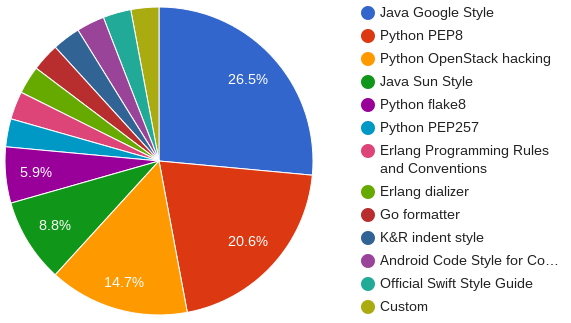
\includegraphics[width=0.5\textwidth]{images/codestyle.png}
\caption{Code style standards followed by INDIGO--DataCloud's software products.}
\label{fig:fig_codestyle}
\end{figure}

Unit testing coverage, another project quality metric, has increased between the first ({\sl INDIGO-1}) and the
second ({\sl INDIGO-2}) INDIGO--DataCloud releases, reaching an average value of
66.69\% on the {\sl INDIGO-2} release, very close to the recommended 70\% threshold
defined by the project’s SQA base criteria \cite{indigo-d31}. A comparison graph
between the code coverage for the products involved both in {\sl INDIGO-1} and
{\sl INDIGO-2} releases is shown in Figure \ref{fig:fig_unittest}. As it can be seen,
a very small set of products with low coverage values highly impacted the overall
result, although a significant part of these products are upstream contributions
or products with codebases not fully under the control of the project. Nevertheless,
60\% of the products were over this threshold while 80\% of them had values above
the 50\% coverage.

The documentation of the products is treated as source code, using a markup
language, automatically rendered and uploaded to online repositories
\cite{indigo-gitbook}. Changes in both documentation and source code are
human--reviewed as the last step before merging them into the production
repository or official documentation.

Last but not least, as described in section \ref{sec:devops}, in order
to facilitate the usage of the INDIGO--DataCloud services, they can be deployed
automatically using either Ansible \cite{indigo-ansible} or Puppet
\cite{indigo-puppet} open--source configuration tools. The adoption of such Configuration Management
tools not only eases the consumption of the products developed by external users or
infrastructures, but also tackles the correct installation and configuration of the
services and applications. A representative example is the \textit{50 roles} being 
developed within the project and currently hosted in the Ansible Galaxy portal for 
the project \footnote{https://galaxy.ansible.com/indigo-dc/}.

\begin{figure*}[ht]
\centering
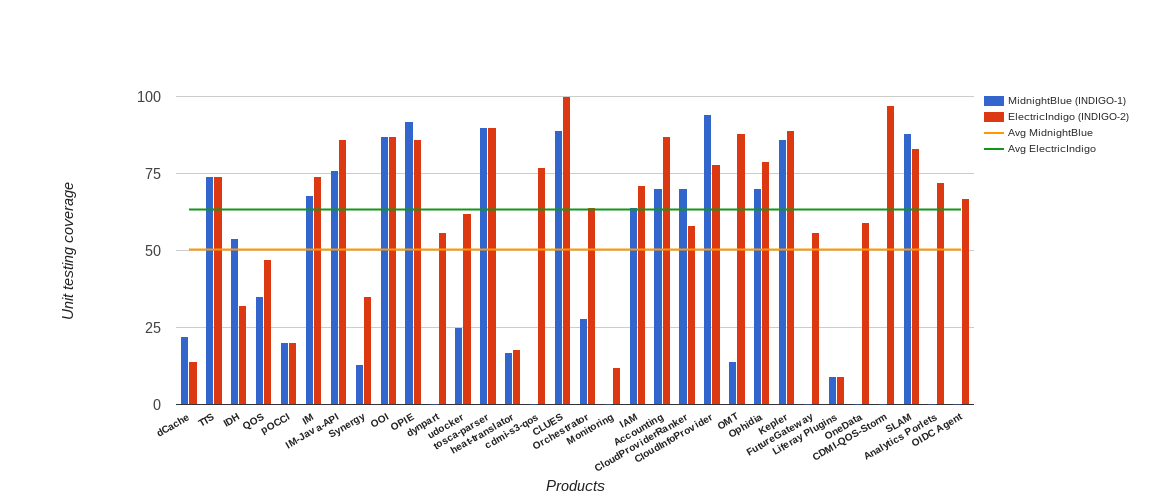
\includegraphics[width=\textwidth]{images/unittest.png}
\caption{Unit testing coverage for the two major INDIGO--DataCloud releases.}
\label{fig:fig_unittest}
\end{figure*}

Figure \ref{fig:fig_confman} shows the number of products that offer an automated means
for deployment. It shows an increase after the {\sl INDIGO-1} release especially
in the previous weeks of each of the two major releases.

The evaluation of the software quality is performed by measuring the values of
the metrics and Key Performance Indicators (KPIs) defined based upon the
ISO/IEC 9126 standard. These metrics cover the development, release and
maintenance phases of the software lifecycle. Development and release metrics
are obtained automatically from several sources, such as GitHub and Jenkins CI
service, and graphically displayed as GitHub pages using GrimoireLab framework
\cite{grimoirelab}. Maintenance and user support metrics are collected from the
different sources of data such as GGUS \cite{ggus} and Github Issues.

\subsection{DevOps practices}
\label{sec:devops}

The DevOps methods emphasize on exercising SQA techniques to avoid infrastructure
disruption whenever new developments are deployed into production systems. The 
following DevOps approaches have been progressively adopted throughout the project's
lifetime, being one of its major outcomes.

\subsubsection{Continuous Integration}
\label{subsec:ci}
The INDIGO--DataCloud project promoted the application of a CI scenario to enforce
the SQA requirements -- described in Section \ref{subsec:sqa} -- for any piece of
software being produced within the project. Such environment requires an automation
ready--to--go infrastructure where the different technologies involved -- source code
management platform, automation server and containerization -- interact with each
other to trigger the source code validation pipeline for each candidate change. The
pipeline is comprised of diverse quality checks, enforcing at least the successful
execution of code style and minimum unit testing coverage. To take over the 
implementation of such infrastructure, the project leveraged on tightly integrated open
source tools such as GitHub \cite{github}, as the online source code repository,
and Jenkins \cite{jenkins}, the event-response CI system. Docker container provisioning
is used to provide instant computing power needed for executing the pipeline jobs. 

This CI approach is guiding the project’s software development phase throughout the
first and second major releases.

\subsubsection{Continuous Delivery}
As DevOps suggests, frequent releases positively affect the reliability of the
software. The software updates of INDIGO--DataCloud products taking place since
the second major release are passing through a Continuous Delivery (CD)
pipeline that adds the packaging of the software right after the successful execution of
the quality checks (as part of the CI). 
The steps defined within the CD pipeline differ whether the software is to be distributed via Docker
images (see Figure \ref{fig:fig_CD}) or via operating system’s packages, rpms or debs. In the latter case an extra
validation step is added, consisting in the product’s deployment using a
Configuration Management (CM) solution. The installation uses the packages
built in the previous step and uploaded to a testing
repository. In the case of Docker images, the CM is used to build the image
itself, installing and configuring the product before uploading it to the
DockerHub repository \cite{indigo-dockerhub}. 


\begin{figure*}[ht]
\centering
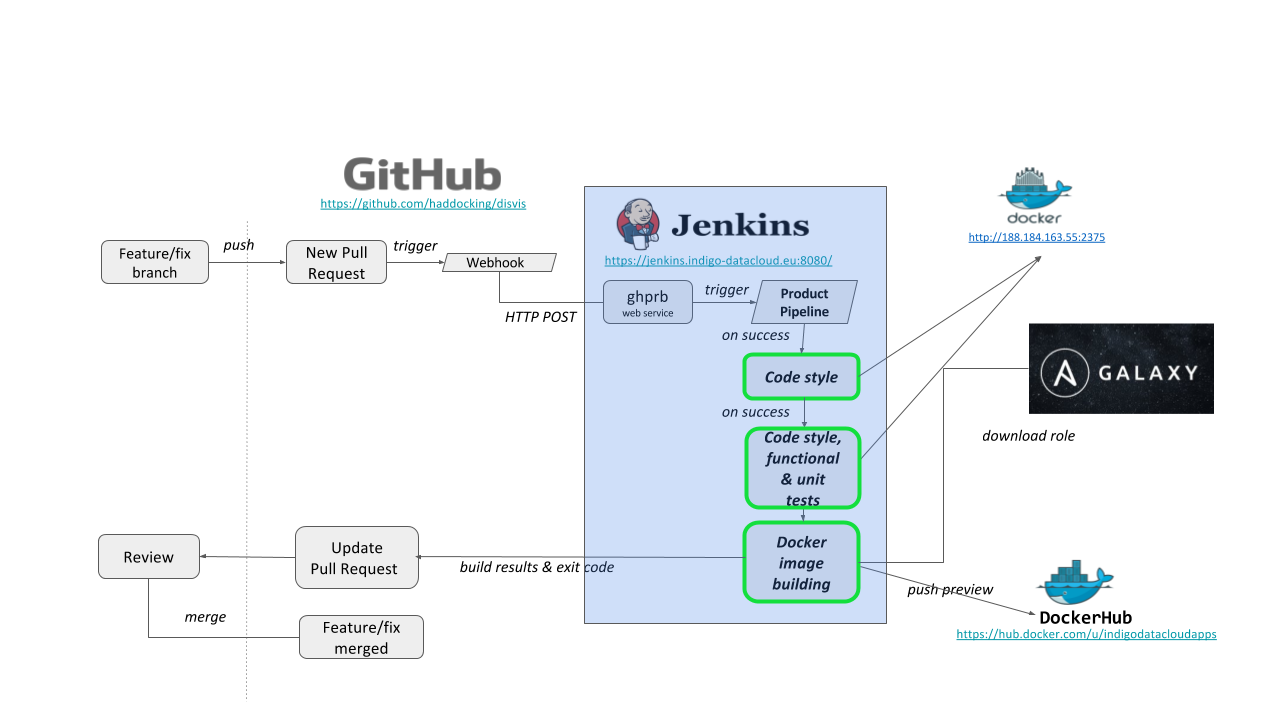
\includegraphics[width=\textwidth]{images/devops.png}
\caption{Continuous Delivery workflow for Docker images.}
\label{fig:fig_CD}
\end{figure*}


\begin{figure}[ht]
\centering
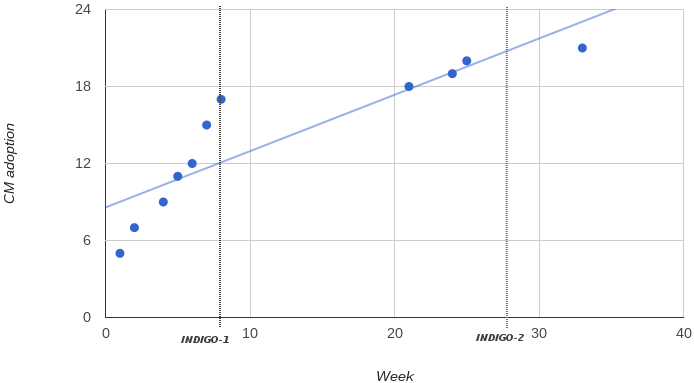
\includegraphics[width=0.45\textwidth, height=50mm]{images/confman.png}
\caption{Trend line showing the adoption of Configuration Management tools throughout the project lifetime.}
\label{fig:fig_confman}
\end{figure}

\begin{figure*}	
	\centering
	\begin{subfigure}
		\centering
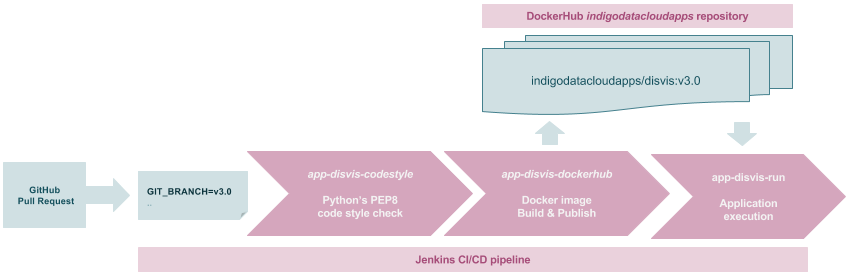
\includegraphics[width=0.85\textwidth]{images/disvis-flow.png}
\caption{DevOps pipeline to distribute Docker images for Disvis application.}
\label{fig:fig_disvis}		
	\end{subfigure}
	\quad
	\begin{subfigure}
		\centering
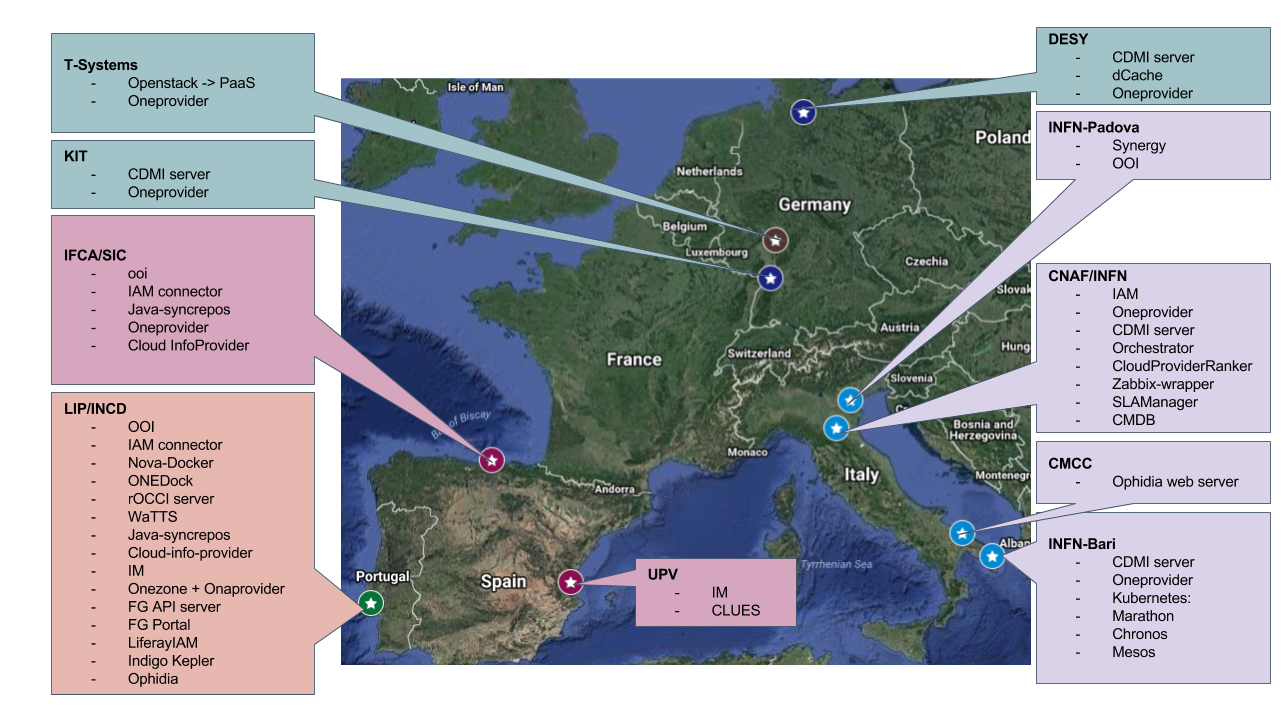
\includegraphics[width=\textwidth]{images/pilotpreview.png}
\caption{Resource centers supporting the Pilot Preview testbed and corresponding
set of deployed INDIGO-DataCloud components or services.}
\label{fig:fig_pilotpreview}
	\end{subfigure}
\end{figure*}


\subsubsection{DevOps adoption from user communities}

The experience gathered throughout the project with regard to the adoption of
different DevOps practices is not only useful and suitable for the software related
to the core services in the INDIGO-DataCloud solution, but also applicable to the
development and distribution of the applications coming from the user communities.

Two applications from "Definition of Support to Research Communities" workpackage, 
DisVis \cite{disvis} and PowerFit \cite{powerfit}, were
integrated into a similar CI/CD pipeline described in section \ref{sec:devops}.
Figure \ref{fig:fig_disvis} shows the pipeline for the Disvis application.

User application developers were provided with both a means to validate the
source code before merging and the creation of a new versioned Docker image,
automatically available in the INDIGO-DataCloud’s application repository.

The novelty introduced in the pipeline above is the validation of the application.
Once the application is packaged as a Docker image, and subsequently uploaded
to the Dockerhub repository, it is instantiated in a new container to be validated.
The application is then executed and the results compared with a set of reference outputs.
Thus this pipeline implementation goes a step forward by testing the application
execution for the latest available Docker image in the catalogue.


\subsection{Integration, preview and early adoption}

Two pilot infrastructures are at the disposal of developers and scientific
communities involved in the project. The aim of these testbeds is to test the
level of integration between the components involved in the INDIGO--DataCloud
solutions and use cases validation, by deploying and executing the applications
with the last stable version of the software in environments as similar as 
possible to production ones. A map of the Pilot Preview
infrastructure is depicted in Figure \ref{fig:fig_pilotpreview}, it shows the
resources providers and the components or services they deployed and supported.


The released software is tested in production environments through the
Staged--Rollout process, before inclusion in the EGI's CloudManagement Distribution (CMD). 
Selected resource providers are requested to install
the most updated stable versions of the software, and to give access to them to their users. The
Staged--Rollout process is key to detect and mitigate issues that could only
appear in production environments.

\section{Conclusion}
\label{sec:con}

It is a fact that the European software produced for scientific purposes is
evolving to a more sustainable model where the quality and reliability of
software is being prioritized. Recent software engineering insights, such as
DevOps approaches, are gradually being applied as the open--source collaborative tools
evolve, allowing tighter integrations. The Software Quality
Assurance procedures have been integrated in the development stage, in order to
detect and correct issues early in the software lifecycle. Automation and
metrics analysis are at the base of prompt issue solving. However, post--release
validation, through the preview testbeds or the Staged--rollout process, are
also needed to strengthen the software reliability for scientific usage.

\section*{Acknowledgment}

The authors would like to thanks European Commission with the various funded
projects.

\begin{thebibliography}{1}

\bibitem{zhu}
L. Zhu and L. Bass and G. Champlin-Scharff, \emph{DevOps and Its Practices},
IEEE Software, vol. 33, no. 3, pp. 32--34, May-June 2016.


\bibitem{cordis:datagrid}
\emph{DataGrid project}, European Community Research and Development
Information Service (CORDIS),
http://cordis.europa.eu/project/rcn/53665\_en.html

\bibitem{globus}
I. Foster and C. Kesselman, \emph{Globus: a Metacomputing Infrastructure
Toolkit}, International Journal of Supercomputer Applications, vol. 11, no. 2,
pp. 115–128, 1997.

\bibitem{datagrid}
L. Momtahan and A. Martin, \emph{e-Science Experiences: Software Engineering
Practice and the EU DataGrid}, in Proc. Asia-Pacific Software Engineering
Conference, Gold Coast, Queensland, Australia, pp. 269-275, IEEE Press,
4-6 Dec. 2002.

\bibitem{agile-manifesto}
\emph{Manifesto for Agile Software Development}, http://agilemanifesto.org

\bibitem{agile}
T. Dingsoyr, \emph{A decade of agile methodologies: Towards explaining agile
software development} in The Journal of Systems and Software, Elsevier Inc,
2012.

\bibitem{cmm}
Paulk et al., \emph{Capability maturity model for software}, Software
Engineering Institute, report CMU/SEI-93-TR-24, ESC-TR-93-177, Feb. 1993.

\bibitem{cordis:egee}
\emph{Enabling Grids for E-sciencE (EGEE)} project, European Community
Research and Development Information Service (CORDIS),
http://cordis.europa.eu/project/rcn/80149\_en.html

\bibitem{cordis:egee2}
\emph{Enabling Grids for E-sciencE-II (EGEE-II)} project, European Community
Research and Development Information Service (CORDIS),
http://cordis.europa.eu/project/rcn/99189\_en.html

\bibitem{cordis:egee3}
\emph{Enabling Grids for E-sciencE-III (EGEE-III)} project, European Community
Research and Development Information Service (CORDIS),
http://cordis.europa.eu/project/rcn/87264\_en.html

\bibitem{egee:acceptance-criteria}
\emph{Definition and Documentation of the Revised Software Life-Cycle Process},
Milestone MSA3.4.2, 2010, EGEE-III project,
https://edms.cern.ch/ui/file/1062487/2/EGEE-III-MSA3.4.2-1062487-v1\_4.pdf

\bibitem{glite}
E. Laure et al, \emph{Programming the Grid with gLite}, in Jin, H., Reed, D.A.,
Jiang, W. (eds.) Computational Methods in Science and Technology, vol. 12(1),
pp. 33–45, Scientific Publishers OWN, 2006.

\bibitem{condor}
D. Thain, T. Tannenbaum, M. Livny, \emph{Condor and the Grid}, in Grid
Computing: Making the Global Infrastructure a Reality, Chapter 11, pp. 63–70,
Eds. John Wiley \& Sons Inc., 2002.

\bibitem{cordis:etics}
\emph{E-Infrastructure for Testing, Integration and Configuration of Software
(ETICS)} project, European Community Research and Development Information
Service (CORDIS), http://cordis.europa.eu/project/rcn/80138\_en.html

\bibitem{cordis:etics2}
\emph{E-Infrastructure for Testing, Integration and Configuration of Software -
Phase 2 (ETICS 2)} project, European Community Research and Development
Information Service (CORDIS),
http://cordis.europa.eu/project/rcn/86604\_en.html

\bibitem{etics}
A. Di Meglio, M.-E.Bégin, P. Couvares, E. Ronchieri, E. Takacs, \emph{ETICS:
the international software engineering service for the Grid}, in Journal of
Physics: Conference Series, Vol. 119, N. 4, IOP Publishing Ltd, 2008.

\bibitem{cordis:emi}
\emph{European Middleware Initiative (EMI)} project, European Community
Research and Development Information Service (CORDIS),
http://cordis.europa.eu/project/rcn/95311\_en.html

\bibitem{iso-9126}
\emph{ISO/IEC 9126 Software Engineering - Product Quality}, International
Organization for Standarization, https://www.iso.org/standard/22749.html

\bibitem{emi-metrics}
\emph{EMI Metrics Specification}, https://goo.gl/CCtY7x


\bibitem{emi-quality-model}
\emph{EMI Quality Model}. Available: https://goo.gl/LdS6fL

\bibitem{cordis:egi-inspire}
\emph{European Grid Initiative: Integrated Sustainable Pan-European
Infrastructure for Researchers in Europe (EGI-InSPIRE)} project, European
Community Research and Development Information Service (CORDIS),
http://cordis.europa.eu/project/rcn/95923\_en.html

\bibitem{egi-ops}
\emph{EGI Operations Portal},
https://operations-portal.egi.eu/

\bibitem{ggus}
\emph{GGUS} EGI Helpdesk,
https://ggus.eu/

\bibitem{gocdb}
\emph{GOCDB} EGI Grid Configuration Repository,
https://ggus.eu/

\bibitem{github}
\emph{GITHUB},
https://github.com/

\bibitem{jenkins}
\emph{Jenkins} Continuous Integration System,
https://jenkins-ci.org/

\bibitem{egi-qc}
\emph{EGI Quality Criteria}. Available: http://egi-qc.github.io/

\bibitem{mario}
M. David et al, \emph{Validation of Grid Middleware for the European Grid
Infrastructure}, in Journal of Grid Computing, vol. 12, issue 3, pp. 543–558,
Springer, 2014.

\bibitem{cordis:egi-engage}
\emph{Engaging the EGI Community towards an Open Science Commons (EGI-ENGAGE)}
project, European Community Research and Development Information Service
(CORDIS), http://cordis.europa.eu/project/rcn/194937\_en.html

\bibitem{cordis:indigo}
\emph{INtegrating Distributed data Infrastructures for Global ExplOitation
(INDIGO-DataCloud)} project, European Community Research and Development
Information Service (CORDIS),
http://cordis.europa.eu/project/rcn/194882\_en.html

\bibitem{indigo-dockerhub}
\emph{INDIGO-DataCloud DockerHub repository},
https://hub.docker.com/u/indigodatacloud

\bibitem{indigo-d31}
\emph{Initial Plan for WP3} INDIGO-DataCloud Deliverable 3.1,
https://www.indigo-datacloud.eu/documents/initial-plan-wp3-d31

\bibitem{indigo-jenkins}
\emph{INDIGO-DataCloud Jenkins CI service},
https://jenkins.indigo-datacloud.eu:8080/

\bibitem{indigo-github}
\emph{INDIGO-DataCloud GitHub Source Code repository},
https://www.github.com/indigo-dc

\bibitem{indigo-gitbook}
\emph{INDIGO-DataCloud GitBook Documentation repository},
https://www.gitbook.com/@indigo-dc

\bibitem{indigo-puppet}
\emph{INDIGO-DataCloud PuppetForge repository},
https://forge.puppet.com/indigodc

\bibitem{indigo-ansible}
\emph{INDIGO-DataCloud Ansible Galaxy repository},
https://galaxy.ansible.com/indigo-dc/

\bibitem{grimoirelab}
\emph{GrimoireLab}, http://grimoirelab.github.io/

\bibitem{ggus}
\emph{Global Grid User Support (GGUS)}, https://www.ggus.eu/

\bibitem{disvis} G.C.P. Van Zundert, A.M.J.J. Bonvin,
DisVis: quantifying and visualizing the accessible interaction space of distance
restrained biomolecular complexes, Bioinformatics 31 (2015) 3222–3224

\bibitem{powerfit} G.C.P. Van Zundert, A.M.J.J. Bonvin,
Fast and sensitive rigid-body fitting into cryo-EM density maps with PowerFit,
AIMS Biophys. 2 (2015) 73–87.

\end{thebibliography}

\begin{IEEEbiography} [{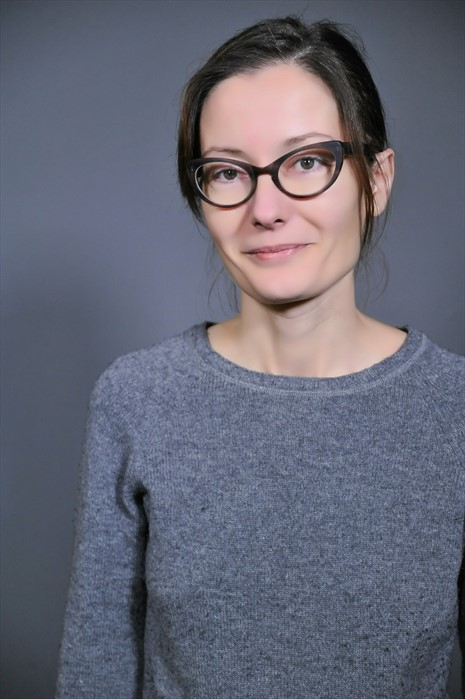
\includegraphics[width=1in,height=1.25in,clip,keepaspectratio]{images/Ronchieri}}]{Elisabetta Ronchieri}
is a Computer Science Engineer at INFN (Istituto Nazionale di Fisica Nucleare - National Institute of Nuclear Physics) CNAF. She holds a PhD in Automation, Robotics and Bioengineering from the University of Pisa. Her main area of interest include software engineering issues, such as software quality and software prediction model. She is also interested in (big and open) data analysis by using techniques coming from various theories, such as Machine Learning.
\end{IEEEbiography}

% if you will not have a photo at all:
\begin{IEEEbiography}[{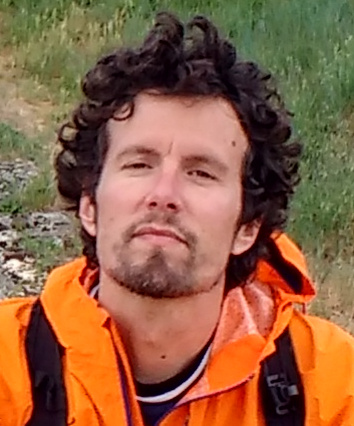
\includegraphics[width=1in,height=1.25in,clip,keepaspectratio]{images/pablo-orviz}}]{Pablo Orviz Fernandez}
is a computing researcher at CSIC (Consejo Superior de Investigaciones
Cientificas), holding an MSc in Scientific Computing from the University of
Cantabria. During the past years he has been devoted to software quality
assurance tasks within different European advanced computing research projects
such as INDIGO-DataCloud and EGI-Engage. Currently involved in EOSC-hub project
and participating in the software quality work packages of DEEP-HybridDataCloud
and eXtreme-DataCloud.
\end{IEEEbiography}

\begin{IEEEbiography}[{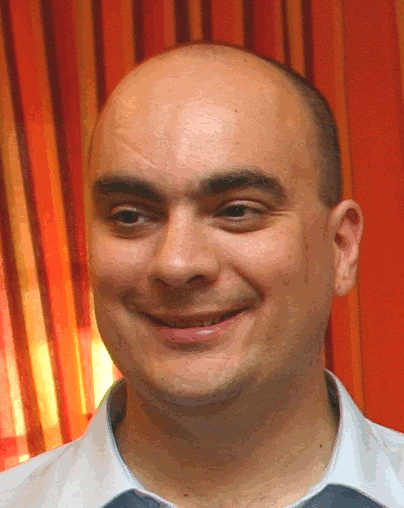
\includegraphics[width=1in,height=1.25in,clip,keepaspectratio]{images/mario-david}}]{Mario David}
is a research associate at LIP. He holds a PhD in Experimental Particle Physics from the University of Lisbon.
Member of DEEP-HybridDataCloud project as Work Package leader of Testbed and integration with EOSC services. Member of EOSC-hub project and
of the Portuguese National Computing Distributed Infrastructure.
He held a research associate position at Institut de Physique du Globe de Paris (IPGP/CNRS) as Scientific Software Developer for the VERCE project, in particular in the data intensive use cases for seismology.
He was been actively involved in the Validation, Quality Assurance and testing of middleware, in regional and global operations.
\end{IEEEbiography}

\begin{IEEEbiography}[{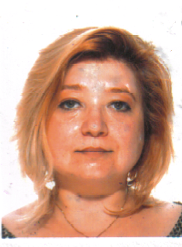
\includegraphics[width=1in,height=1.25in,clip,keepaspectratio]{images/cris_foto_good}}]{Doina Cristina Duma}
is the leader of the Distributed Systems group at the INFN National Center (CNAF), providing the core operational support for the INFN-wide Grid infrastructure and for the CNAF Cloud infrastructure. She has a long experience in managing distributed e-infrastructures, being involved since 2003 in major European projects such as DataGrid, EGEE (I, II, III), EGI-Inspire and EGI-Engage. She was the Release Manager of the EMI (European Middleware Initiative) and INDIGO - DataCloud European project project and having as main responsibilities to manage all release activities, including release planning, building, deploying, reporting, establishing and maintaining the overall release timeline and milestones.
\end{IEEEbiography}


\begin{IEEEbiography}[{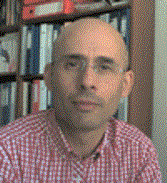
\includegraphics[width=1in,height=1.25in,clip,keepaspectratio]{images/jorge-gomes}}]{Jorge Gomes}
is a computing researcher at LIP. He worked in the development of advanced data acquisition systems at CERN, and participated in pioneering projects in the domain of digital satellite data communications, IP over ATM, and advanced videoconferencing over IP networks. Since 2001 he has participated in numerous projects regarding distributed computing, networks and security in Europe and Latin America. He is the head of the LIP Advanced Computing and Digital Infrastructures Group and technical coordinator of the Portuguese National Grid Infrastructure, representative of Portugal in the Council of the European Grid Infrastructure (EGI) and responsible for the Portuguese participation in IBERGRID, that joins Portuguese and Spanish distributed computing infrastructures.
\end{IEEEbiography}

\begin{IEEEbiography}[{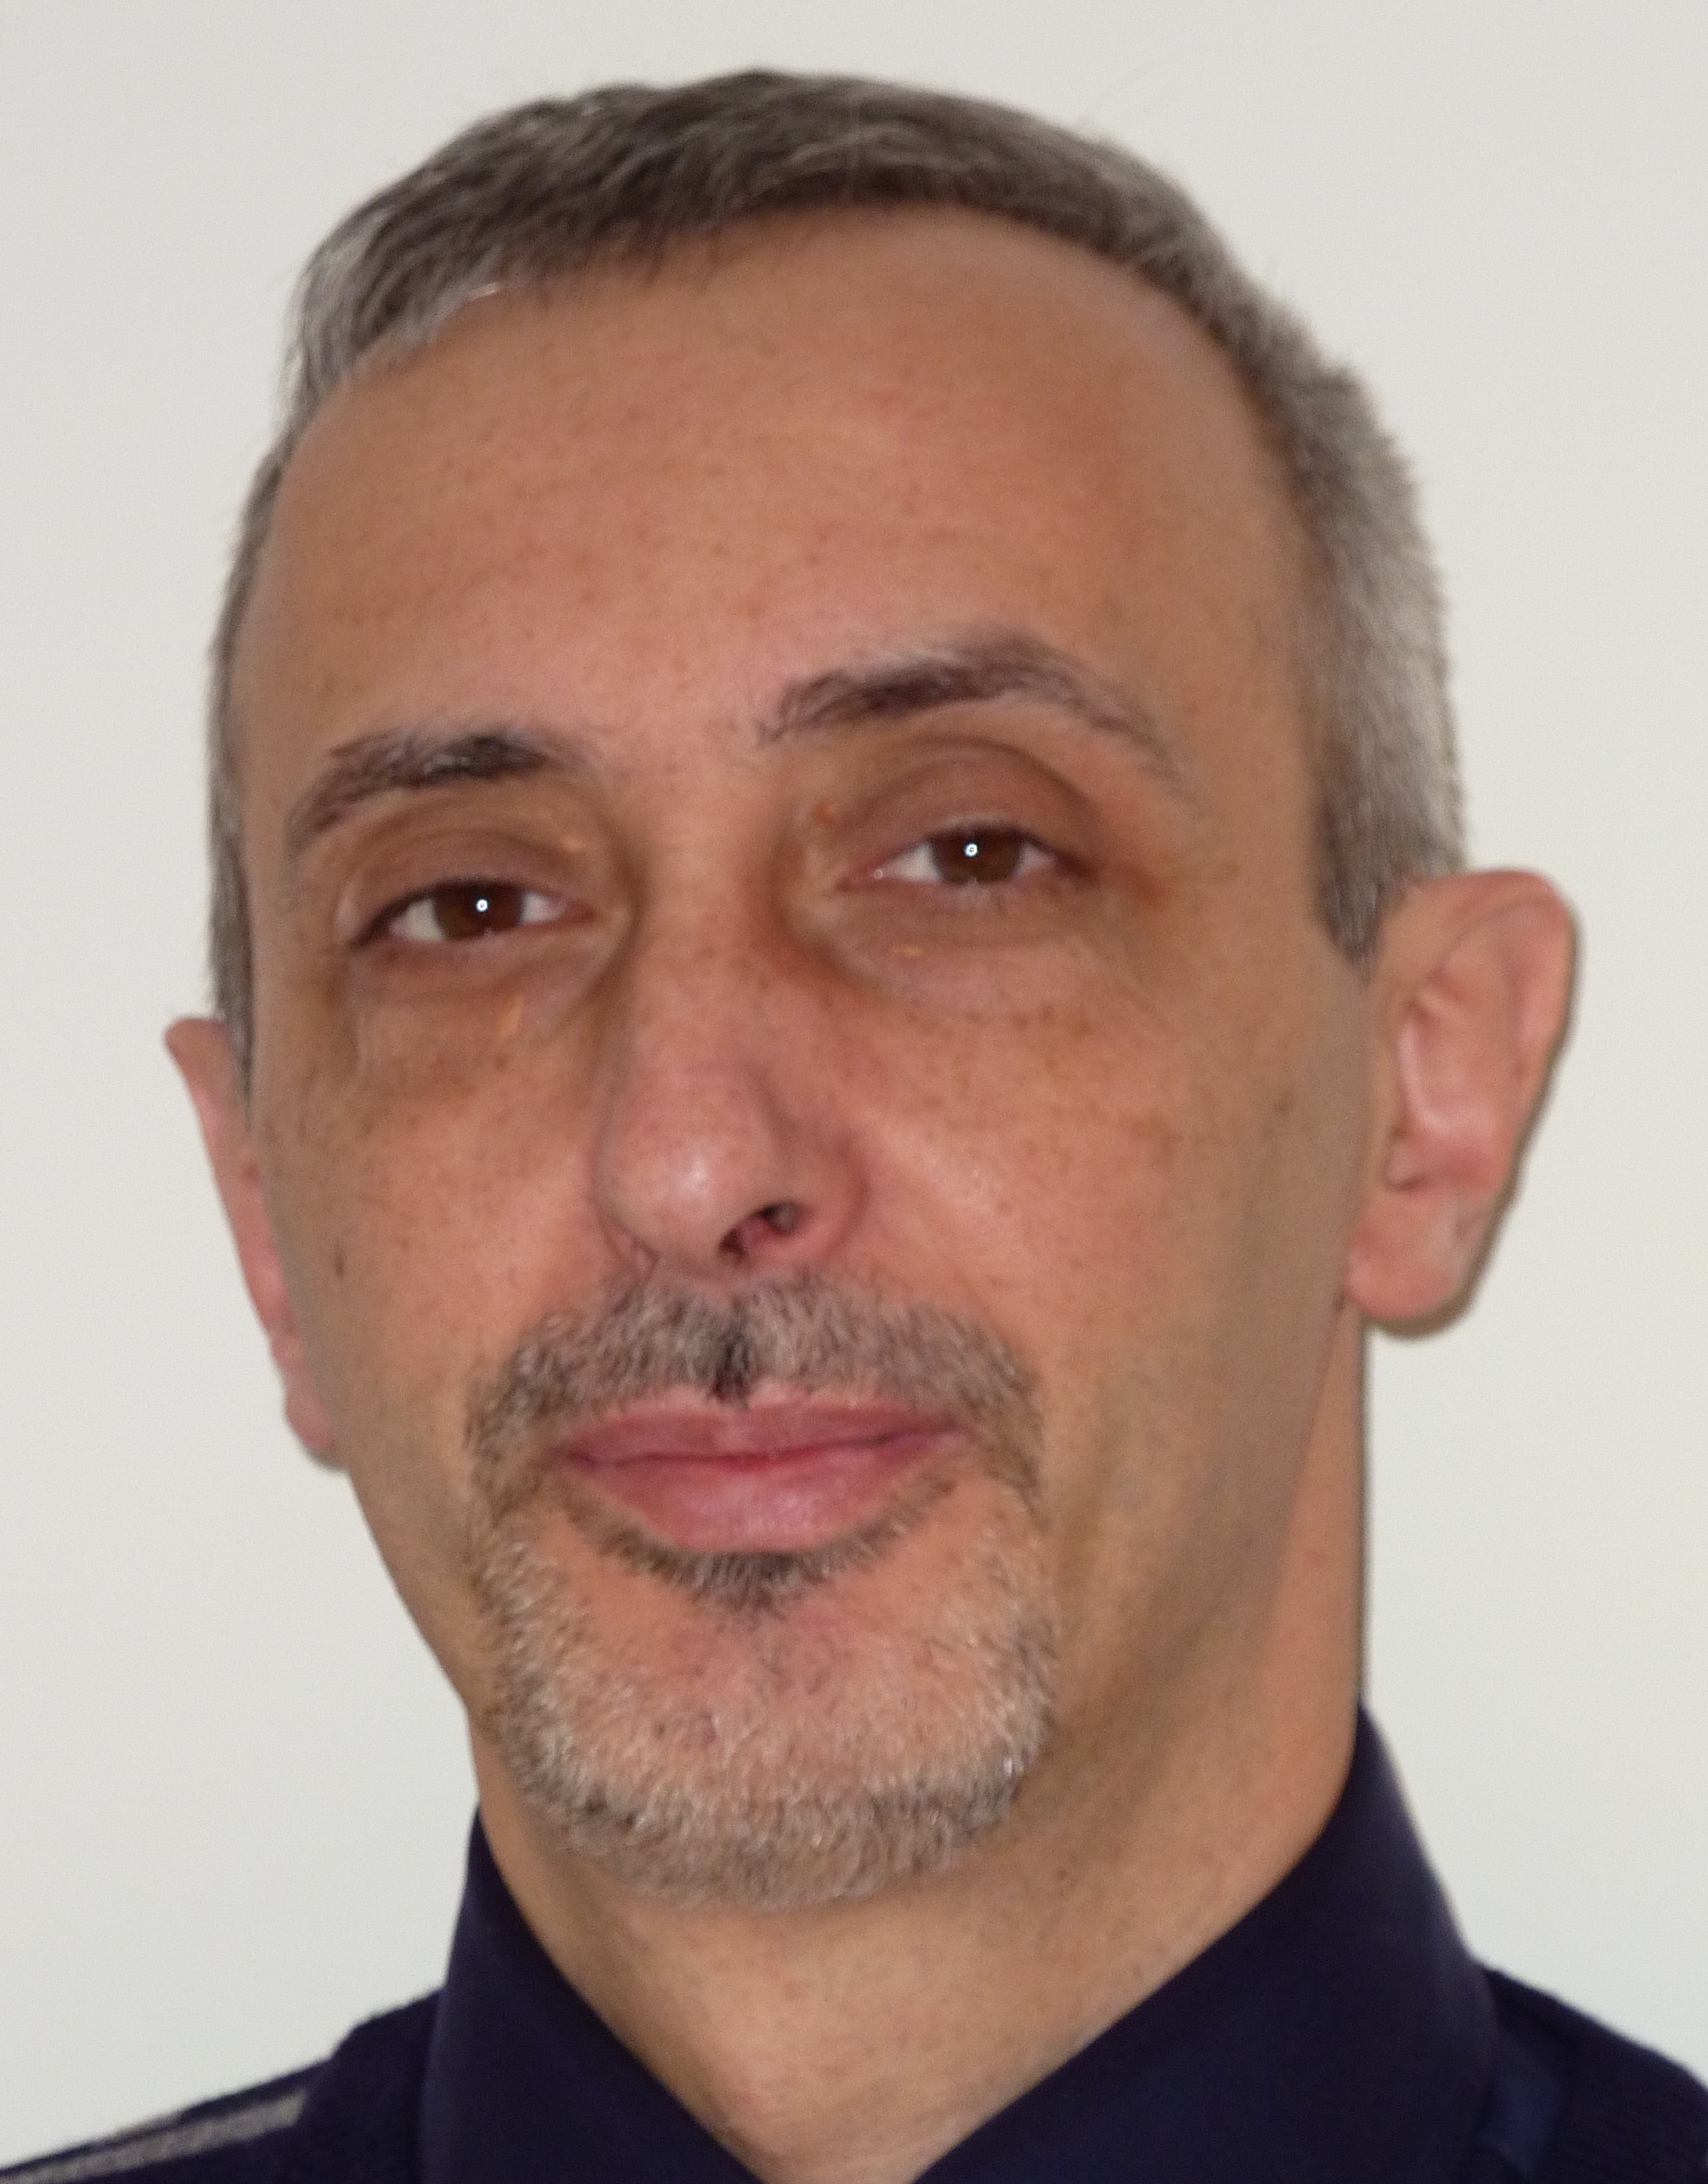
\includegraphics[width=1in,height=1.25in,clip,keepaspectratio]{images/DavideSalomoni}}]{Davide Salomoni}
is Director of Technology at the Italian National Institute for Nuclear Physics (INFN). He has 27 years of international experience in private and public environments related to distributed computing and communication technologies. He currently leads the Software Development and Distributed Systems department at CNAF, the INFN National Center dedicated to research and development on IT technologies, located in Bologna, Italy. He was Project Coordinator of INDIGO-DataCloud, a project funded by the EC Horizon2020, that developed innovative open source computing and storage solutions.
\end{IEEEbiography}





\end{document}


